\documentclass{fisatproject}
\usepackage{comment}
\usepackage{tocloft}
\usepackage{graphicx}
\usepackage{verbatim}
\usepackage[top=0.70in, bottom=0.70in, left=0.8in,right=0.80in]{geometry} % setting the page alignment with this package
\usepackage{array} % for making text bold in table
\usepackage{setspace}
\usepackage{float}
\usepackage{enumerate}
\usepackage{longtable}
\usepackage[font=small,labelfont=bf]{caption} 
\usepackage{tikz}
\title{Social Robot}
\team{Yedhin Kizhakkethara\\Ranjith R.K\\Leo Varghese\\Sandeep Ramesh}
\author{Yedhin Kizhakkethara(FIT16CS125)}
\begin{document}
\maketitle

\makecert

\newpage
\pagenumbering{roman}
\setcounter{page}{1}
\newgeometry{top=4cm,bottom=0.1cm}
\renewcommand\abstractname{ABSTRACT}
\begin{abstract}
\vspace{5cm}
Social Robots soon will be an inevitable part of the distant future in the digital era. A social robot has the ability to see and differentiate the objects in its vision. This feat is achieved by infusing relevant and rather popular computing domains such as Android, Machine learning, Image Processing, Networking etc. Overall, a social robot can imitate certain human features like speaking, movement of head, closing of eyelids and identification of objects in real time. This project aims to create such a social robot which is incorporated with the above mentioned features.
\end{abstract}


\newpage
%\thispagestyle{plain}
\renewcommand\abstractname{ACKNOWLEDGMENT}
\begin{abstract}
\vspace{5cm}
The success and final outcome of this project required a lot of guidance and assistance from many people and I am extremely privileged to have got this all along for completing of the project.\newline\newline

I respect and thank APJ Abdul Kalam Technological University (KTU) for providing me an opportunity to do the project work in my college.\newline\newline

I would like to express my deepest appreciation towards \textbf{Dr. George Issac}, Principal, Federal Institute of Science and Technology (FISAT), \textbf{Dr. Prasad J C},  Head  of  Department, Computer Science and Engineering, for making the college facilities available at all times.\newline\newline

I am profoundly grateful to \textbf{Mr. Mahesh C}, for his expert guidance and continuous encouragement throughout to see that this project reaches its target since its commencement to its completion.\newline\newline

I owe my deepest gratitude to our group advisors \textbf{Ms. Resmi R}, \textbf{Mr. Jestin Joy} and \textbf{Ms. Merin Cherian}, for their guidance and constant supervision as well as for providing necessary information regarding the project.\newline\newline

I am thankful to all other teaching and non-teaching staff for their support in completing the project.\newline\newline

I would also like to thank \textbf{Mr. Pankaj Kumar G}, \textbf{Ms. Soumya S Raj} and \textbf{Mr. Varun P Nair} for helping us out in many aspects of the project and also in setting up the lab for our final presentation.\newline\newline

Last but not the least, I would also like to thank my fellow teammates for their enthusiastic support through coordination and cooperation.
\vspace{1cm}
\begin{flushright}
Yedhin Kizhakkethara
\end{flushright}
\end{abstract}
\newpage

\restoregeometry
\tableofcontents
\newpage

\cleardoublepage
\addcontentsline{toc}{chapter}{\listfigurename}
\listoffigures
\newpage

\cleardoublepage
%\addcontentsline{toc}{chapter}{\listtablename}
\listoftables
\newpage
\pagestyle{fancy}


\chapter{INTRODUCTION}
\pagenumbering{arabic}
\setcounter{page}{1}
\renewcommand{\baselinestretch}{1.50}
\section{Overview}
A social robot is an autonomous robot that interacts and communicates with humans or other autonomous physical agents by following social behaviors and rules attached to its role.

\section{Objective}
The objective of the project is to make a social robot which can enact certain human features like identification of objects seen through its vision, speaking out about the objects which it can see, movement of the head, and closing of eyelids, by making use of popular domains such as android, machine learning, image processing and networking.

\section{Scope Of Project}
The social consequences of robotics depend to a significant degree on how robots are employed by humans, and to another compelling degree on how robotics evolves from a technical point of view.\cite{a} That is why it could be instructive for engineers interested in cooperating with sociologists to get acquainted with the problems of social work and other social services, and for sociologists interested in the social dimensions of robotics to have a closer look at technical aspects of new generation robots.\cite{b}\newline\newline
\par
Interactive robotic toys like Hasbro’s Baby Alive My Real Babies; household companions such as Sony’s AIBO dog, Jetta’s robotic dinosaur Pleo, and Aldebaran’s NAO next generation robot; therapeutic pets like the Paro baby seal; and the Massachusetts Institute of Technology (MIT) robots Kismet, Cog, and Leonardo.\cite{c}The use of humanoid robots to comfort and entertain lonely older persons has already triggered an ethical debate.\cite{e}\newline\newline
\par
The relevance of social robots should not be underestimated. In technologically advanced societies, a process of robotization of social work is already underway.\cite{h} For instance, robots are increasingly used in the care of the elderly. This is a consequence of two other processes occurring simultaneously: on the one hand, we have an aging population with a resulting increase in demand for care personnel; on the other hand, technological developments have created conditions to deal with this problem in innovative ways.

\section{Robotics}
Robotics can be described as the current pinnacle of technical development. Robotics is a confluence science using the continuing advancements of mechanical engineering, material science, sensor fabrication, manufacturing techniques, and advanced algorithms. The study and practice of robotics will expose a dabbler or professional to hundreds of different avenues of study. For some, the romanticism of robotics brings forth an almost magical curiosity of the world leading to creation of amazing machines. A journey of a lifetime awaits in robotics.\cite{f,g}\newline\newline
Robotics can be defined as the science or study of the technology primarily associated with the design, fabrication, theory, and application of robots. While other fields contribute the mathematics, the techniques, and the components, robotics creates the magical end product. The practical applications of robots drive development of robotics and drive advancements in other sciences in turn.

\begin{center}
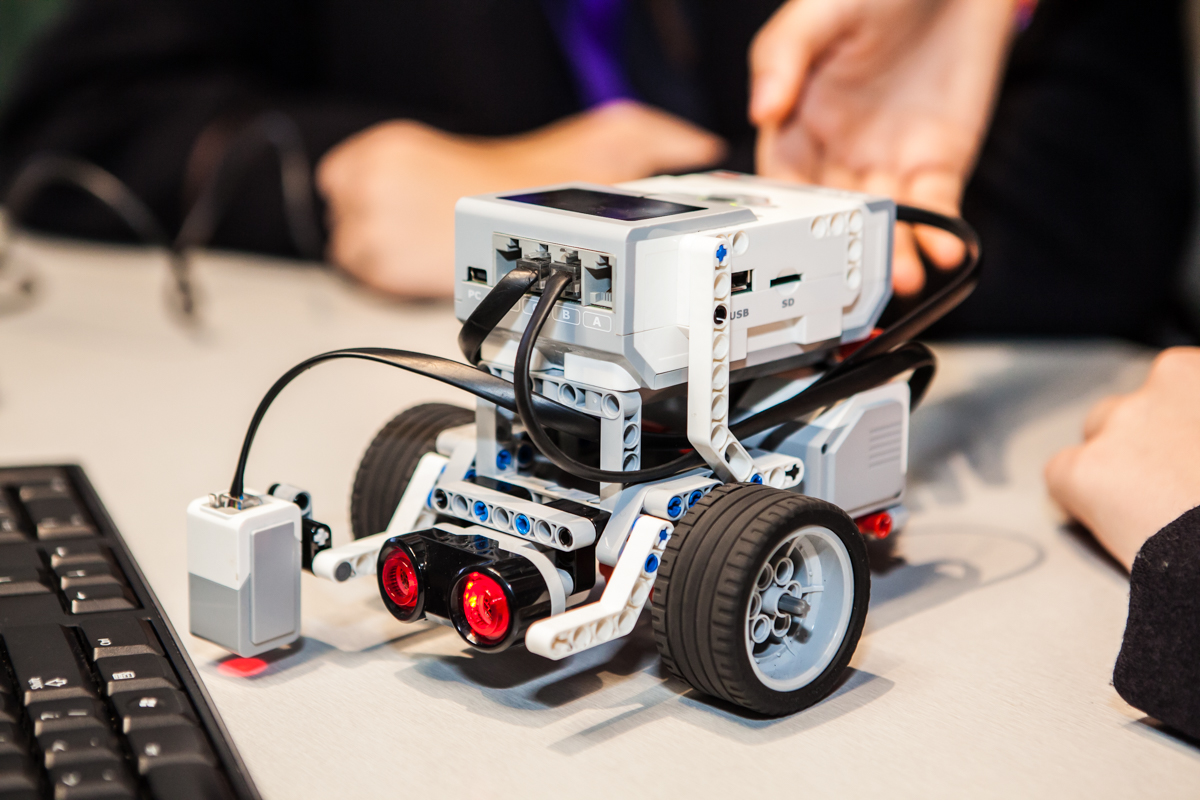
\includegraphics[scale=.2]{robo.png}
\captionof{figure}{Line Follower Robot}
\end{center}

The promise of robotics is easy to describe but hard for the mind to grasp. Robots hold the promise of moving and transforming materials with the same plan and ease as a computer program transforms data. Today, robots mine minerals, assemble semi-processed materials into automobile components, and assemble those components into automobiles. On the immediate horizon are self-driving cars, robotics to handle household chores, and assemble specialized machines on demand.\cite{i,b,c} It is not unreasonable to imagine robots that are given some task, such as reclaim desert into photo-voltaic cells and arable land, and left to make their own way. Then the promise of robotics exceeds the minds grasp.\newline
In summary, robotics is the field related to science and technology primarily related to robotics. It stands tall by standing the accomplishments of many other fields of study.


\section{Characteristics}
Sensing: First of all your robot would have to be able to sense its surroundings. It would do this in ways that are not dissimilar to the way that you sense your surroundings.
\vspace{1cm}

Movement: A robot needs to be able to move around its environment. Whether rolling on wheels, walking on legs or propelling by thrusters a robot needs to be able to move. To count as a robot either the whole robot moves, like the Sojourner or just parts of the robot moves, like the Canada Arm.
\vspace{1cm}

Energy: A robot needs to be able to power itself. A robot might be solar powered, electrically powered, battery powered. The way your robot gets its energy will depend on what your robot needs to do.
\vspace{1cm}

Intelligence: A robot needs some kind of "smarts." This is where programming enters the pictures. A programmer is the person who gives the robot its 'smarts.' The robot will have to have some way to receive the program so that it knows what it is to do.


\section{Application}
Robotics is the engineering science and technology which involves the conception, design, operation and manufacture of robots. Electronics, mechanics and software are brought together by robotic.Robots are used for jobs that are dirty, dull and dangerous. Today robotics have many different application areas. Some of those are:\newline\newline
Outer Space Applications: Robots are playing a very important role for outer space exploration. The robotic unmanned spacecraft is used as the key of exploring the stars, planets...etc.
Sojourner Mars Explorer Robot The most famous robots used in the outer space applications are the Mars rovers of NASA. In 1997 The Pathfinder Mission landed on Mars. Its robotic rover Sojourner, rolled down a ramp and onto Martian soil in early July. It continued to broadcast data from the Martian surface until September.
Sojourner performed semi-autonomous operations on the surface of Mars as part of the Mars Pathfinder mission; equipped with an obstacle avoidance program. Sojourner was capable of planning and navigating routes to study the surface of the planet. Sojourner's ability to navigate with little data about its environment and nearby surroundings allowed the robot to react to unplanned events and objects.\cite{i}

\begin{center}
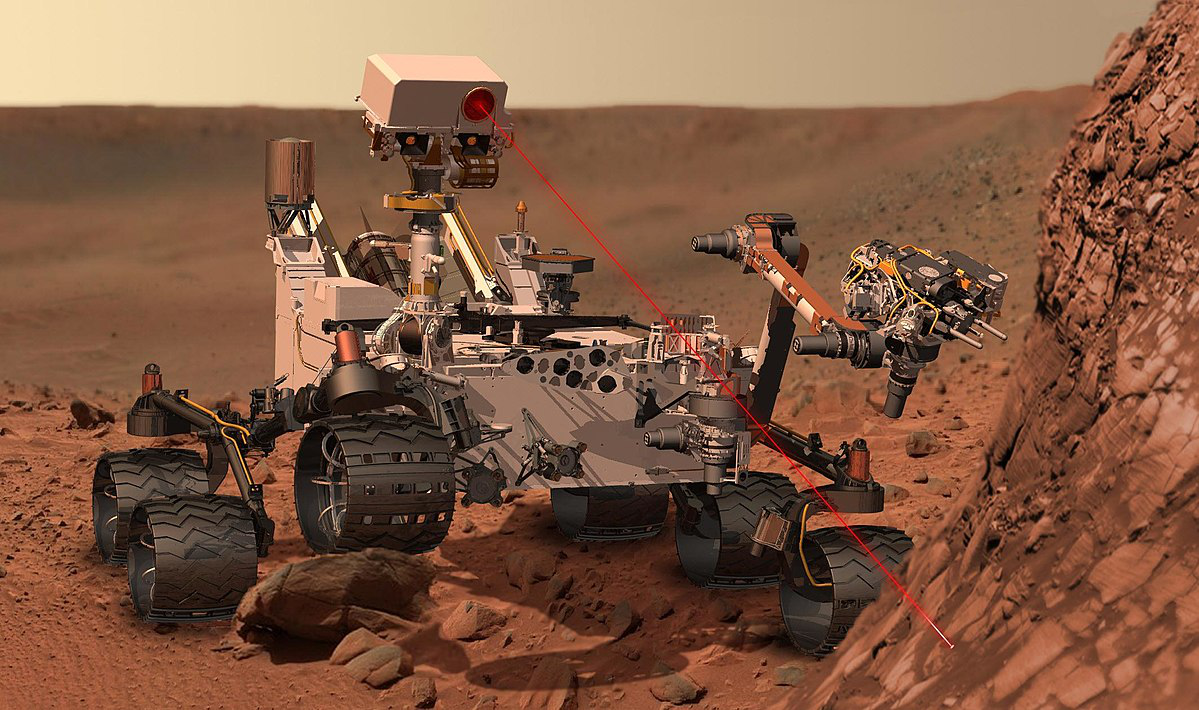
\includegraphics{mars.png}
\captionof{figure}{NASA Mars Rover}
\end{center}

Spirit and Opportunity Mars Rovers After Sojourner's mission NASA sent twin robots Spirit and Opportunity to the Red Planet on 10, June and 23, July 2003. Spirit and Opportunity landed on Mars on 4, January and 25, January 2004. 
Spirit and Opportunity are solar powered robots with six wheels included their own motors. Both of the Mars Rovers are 1,5 m high, 2,3 m wide and 1,6 m long and weighing 180 kg. Spirit and Opportunity have many science instruments in order to perform their missions on Mars. They have a robot arm, that contains a Mössbauer spectrometer to investigate the mineralogy of the rocks and soils on Mars, an Alpha particle X-ray spectrometer for analysis of elements found in rocks and soils, a rock abrasion tool used to expose the fresh material for examination, a microscopic image and magnets to collect magnetic particles.
Phoenix Mars Explorer Robot The twin Mars Rovers have a panoramic camera used for examinations of the texture, color, mineralogy, and structure of the local terrain, a miniature thermal emission spectrometer for identification promising rocks and soils which is useful to determine the formation processes of them. There is also a navigation camera on both Mars rovers in order to take view with a higher field but lower resolution for driving and navigation.\cite{j,k}
Phoenix Mars Rover was sent to the Red Planet on 4, August 2007 and landed on 25, May 2008. The mission of the Phoenix was to investigate the existence of water and life supporting conditions on Mars.

\vspace{1cm}
Military Applications: In today's modern army robotics is an important factor which is researched and developed day by day. Already remarkable success has been achieved with unmanned aerial vehicles like the Predator drone, which are capable of taking surveillance photographs, and even accurately launching missiles at ground targets, without a pilot. There are many advantages in robotic technology in warfare however, as outlined by Major Kenneth Rose of the US Army's Training and Doctrine Command: ''Machines don't get tired. They don't close their eyes. They don't hide under trees when it rains and they don't talk to their buddies...A human's attention to detail on guard duty drops dramatically in the first 30 minutes ... Machines know no fear.''

\begin{center}
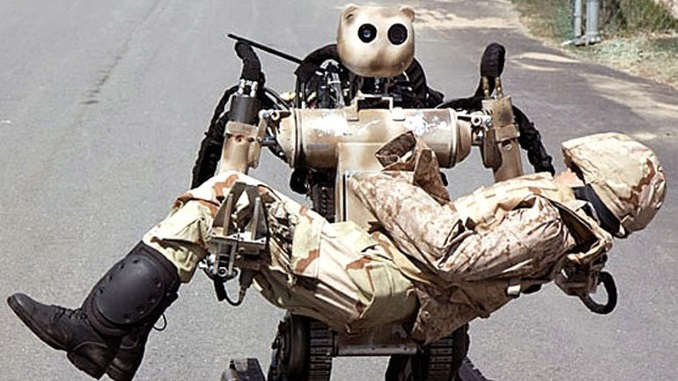
\includegraphics[scale=.5]{mil.png}
\captionof{figure}{Robots in Military Field}
\end{center}

Intelligent Home Applications: We can monitor home security, environmental conditions and energy usage with intelligent robotic home systems. Door and windows can be opened automatically and appliances such as lighting and air conditioning can be pre-programmed to activate. This assists occupants irrespective of their state of mobility.

\begin{center}
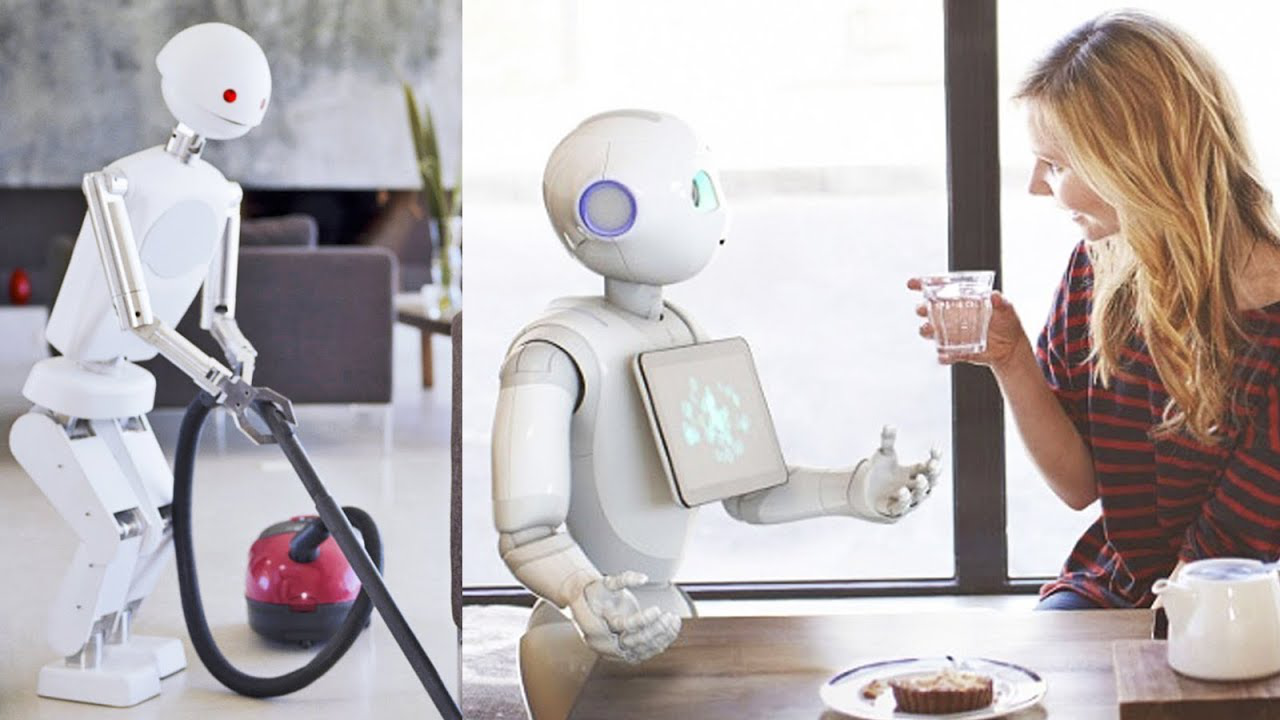
\includegraphics[scale=.3]{home.png}
\captionof{figure}{Robots in Household Applications}
\end{center}

Industry: From the beginning of the industrial revolution robotics and automation becomes the most important part of manufacturing. Robotic arms which are able to perform multiple tasks such as welding, cutting, lifting, sorting and bending are used in fabrics. 
\newpage
\begin{center}
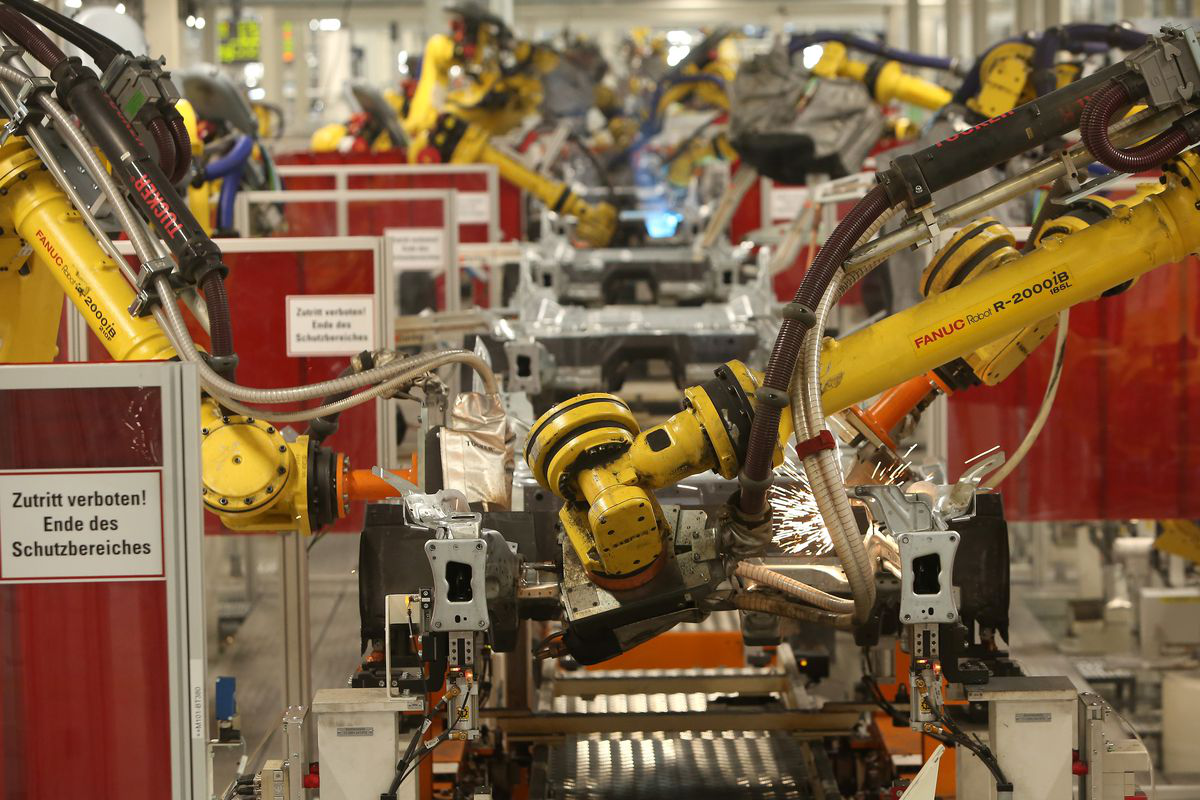
\includegraphics[scale=.3]{ind.png}
\captionof{figure}{Robots in Industrial Applications}
\end{center}

The most commonly used configurations of the industrial robots are:\newline\newline
* Articulated Robots: An articulated robot is one which uses rotary joints to access its work space.  Articulated robots can range from simple two-jointed structures to systems with 10 or more interacting joints.The six-axis, articulated robot is the most versatile industrial robot which allows for a high level of freedom.\newline\newline
* Cylindrical Coordinate Robots: These robots have three degrees of freedom and they moves linearly only along the Y and Z axes with a cylindrical work envelope.\newline\newline
* Scara Robots: It stands for Selective Compliant Assembly Robot Arm or Selective Compliant Articulated Robot Arm. Scara robots usually have four axes as any X-Y-Z coordinate within their work envelope and a fourth axis of motion which is the wrist rotate (Theta-Z).\newline\newline
* Spherical Coordinate Robots: The spherical arm, also known as polar coordinate robot arm, has one sliding motion and two rotational, around the vertical post and around a shoulder joint.\newline\newline
*Cartesian Coordinate Robots: Rectangular arms are sometimes called "Cartesian" because the arm´s axes can be described by using the X, Y, and Z coordinate system. It is claimed that the Cartesian design will produce the most accurate movements.\newline\newline
*Delta Robots: A Delta robot consists of three arms connected to universal joints at the base. The key design feature is the use of parallelograms in the arms, which maintains the orientation of the end effector. The Delta robot has popular usage in picking and packaging in factories.\cite{b}

\vspace{1cm}
Health Service: Under development is a robotic suit that will enable nurses to lift patients without damaging their backs. Scientists in Japan have developed a power-assisted suit which will give nurses the extra muscle they need to lift their patients - and avoid back injuries.\cite{c}

\begin{center}
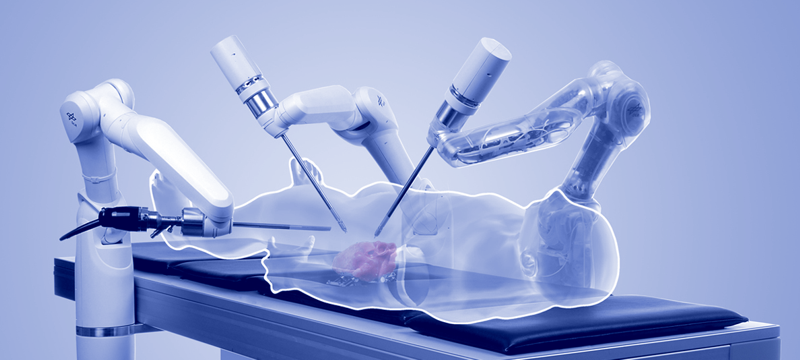
\includegraphics[scale=.5]{heal.png}
\captionof{figure}{Robot in Health Services}
\end{center}

\chapter{RELATED WORK}
\begin{itemize}
\item Kismet

    \begin{itemize}
    \item It’s a robot made at MIT as an experiment in effective
computing.
    \item Kismet simulates emotions through various facial expressions, vocalizations and movement.
    \end{itemize}
\begin{center}
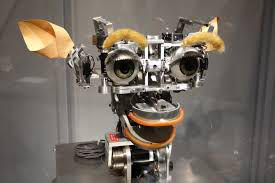
\includegraphics{kismet.png}
\captionof{figure}{Kismet}
\end{center}    

\begin{comment}
Kismet is an expressive robotic creature with perceptual and motor modalities tailored to natural human communication channels. To facilitate a natural infant-caretaker interaction, the robot is equipped with visual, auditory, and proprioceptive sensory inputs. The motor outputs include vocalizations, facial expressions, and motor capabilities to adjust the gaze direction of the eyes and the orientation of the head. Note that these motor systems serve to steer the visual and auditory sensors to the source of the stimulus and can also be used to display communicative cues.
Our hardware and software control architectures have been designed to meet the challenge of real-time processing of visual signals (approaching 30 Hz) and auditory signals (8 kHz sample rate and frame windows of 10 ms) with minimal latencies (less than 500 ms). The high-level perception system, the motivation system, the behavior system, the motor skill system, and the face motor system execute on four Motorola 68332 microprocessors running L, a multi-threaded Lisp developed in our lab. Vision processing, visual attention and eye/neck control is performed by nine networked 400 MHz PCs running QNX (a real-time Unix operating system). Expressive speech synthesis and vocal effective intent recognition runs on a dual 450 MHz PC running NT, and the speech recognition system runs on a 500 MHz PC running Linux.\cite{d}
\end{comment}

\item Joe Robot
    \begin{itemize}
        \item It’s a robot made in research of Anthropomorphism.
        \item It develops intelligence during the meaningful social
interactions between AI and people.
    \end{itemize}
    \newpage
\begin{center}
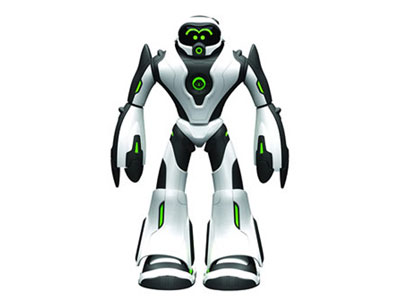
\includegraphics{joe_bot.png}
\captionof{figure}{Joe Robot}
\end{center}    
\item Furby
    \begin{itemize}
        \item It’s a electronic robotic toy created by Tiger Electronics.
        \item Furby initially speaks in furbish and then later on learns the language that the owner speaks by itself.
    \end{itemize}
\end{itemize}
\begin{center}
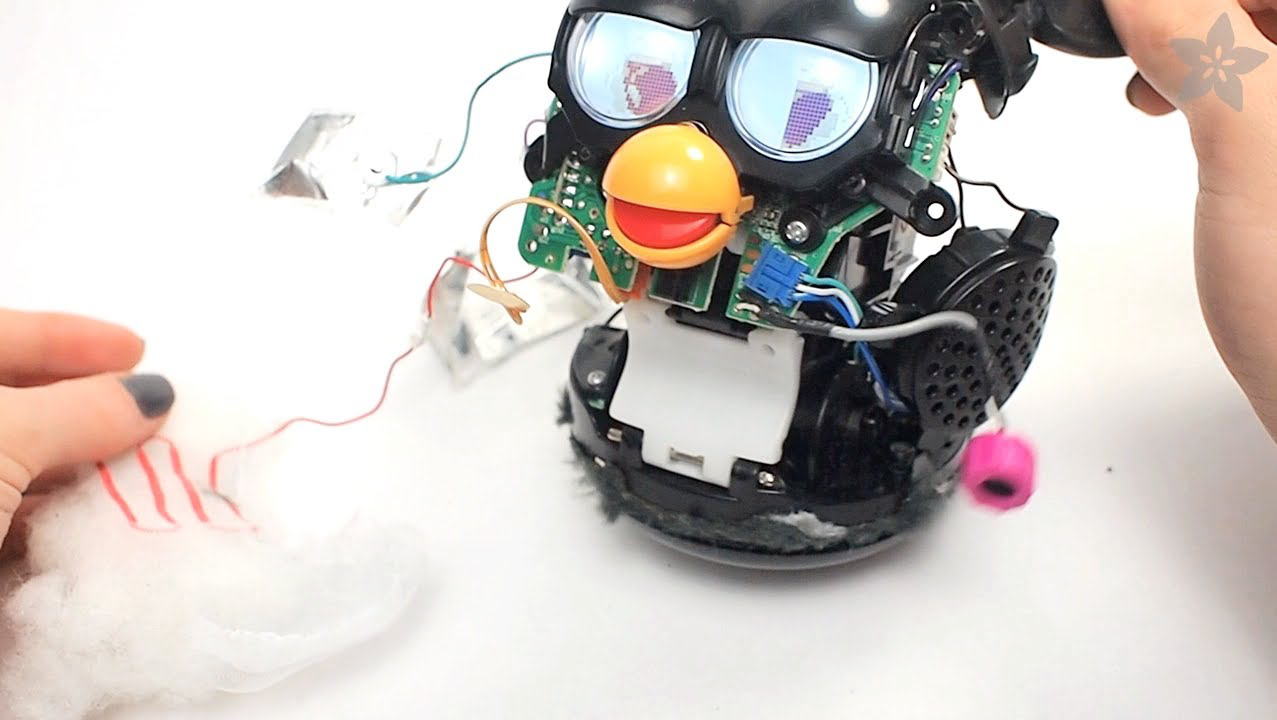
\includegraphics[scale=0.3]{furby.png}
\captionof{figure}{Furby Robot}
\end{center}    
Furby is an American electronic robotic toy released in 1998 by Tiger Electronics. It resembles a hamster or owl-like creature and went through a period of being a "must-have" toy following its holiday season launch, with continual sales until 2000. Over 40 million Furbies were sold during the three years of its original production, with 1.8 million sold in 1998, and 14 million in 1999. Its speaking capabilities were translated into 24 languages.\newline\newline
Furbies were the first successful attempt to produce and sell a domestically-aimed robot. A newly purchased Furby starts out speaking entirely "Furbish", the unique language that all Furbies use, but is programmed to start using English words and phrases in place of Furbish over time. This process is intended to resemble the process of learning English.[1] The updated Emoto-Tronic Furby, with voice-recognition and more complex facial movements, was sold by Hasbro between 2005–2007. They released another updated Furby with LCD eyes and a mobile app for the holiday season in 2012.\cite{e}



\chapter{DESIGN and IMPLEMENTATION}

\section{Design}
The proposed work is to create a social robot which can identify objects in its visibility. The physical body of the robot will have human like movement capabilities, like movement of head, closing of eyelids and speaking. A web camera will act as the eyes of the robot. The live feed from the web camera will be directed to an android app and send via WiFi to the server, where classification will take place. An image classification model trained using Support Vector Machine(SVM) will be used in the process of classification. The prediction will be send back to the android app which would then act as the mouth of the robot and speak out what it sees.
\subsection{UML Deployment Diagram}
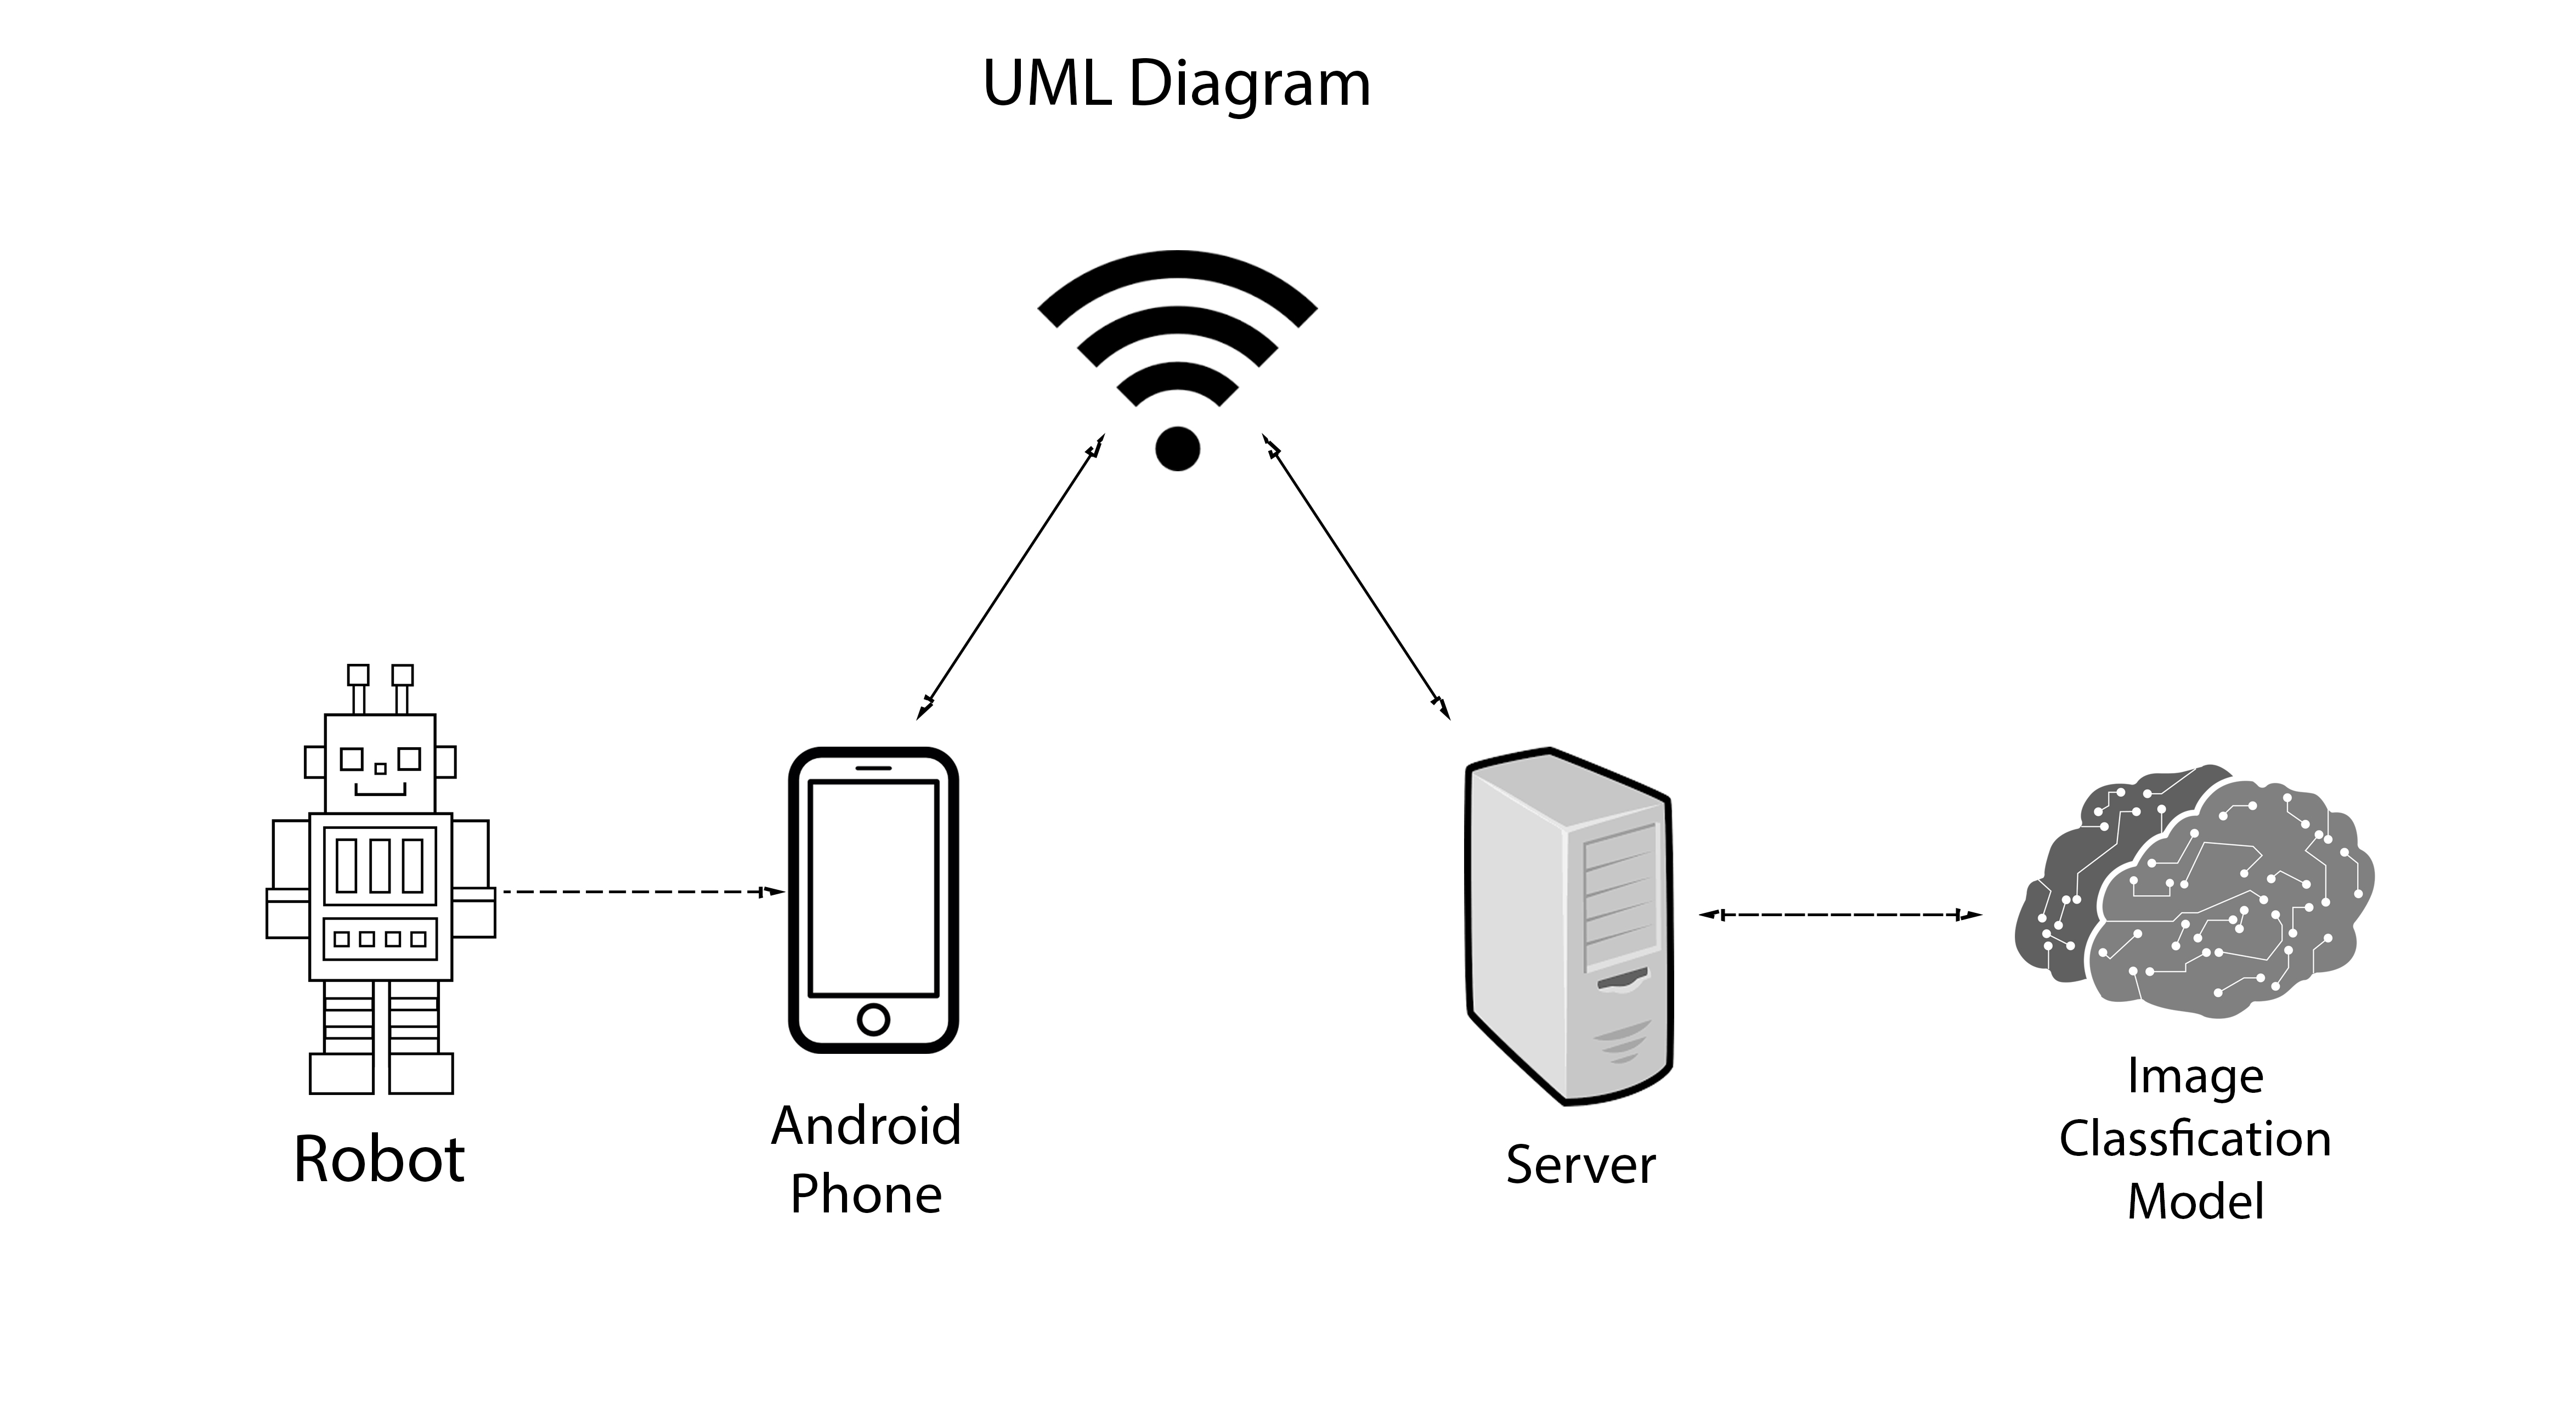
\includegraphics[scale=0.40]{uml_dia.jpg}
\subsection{Data Flow Diagram - Level 0}
\begin{flushleft}
\centerline{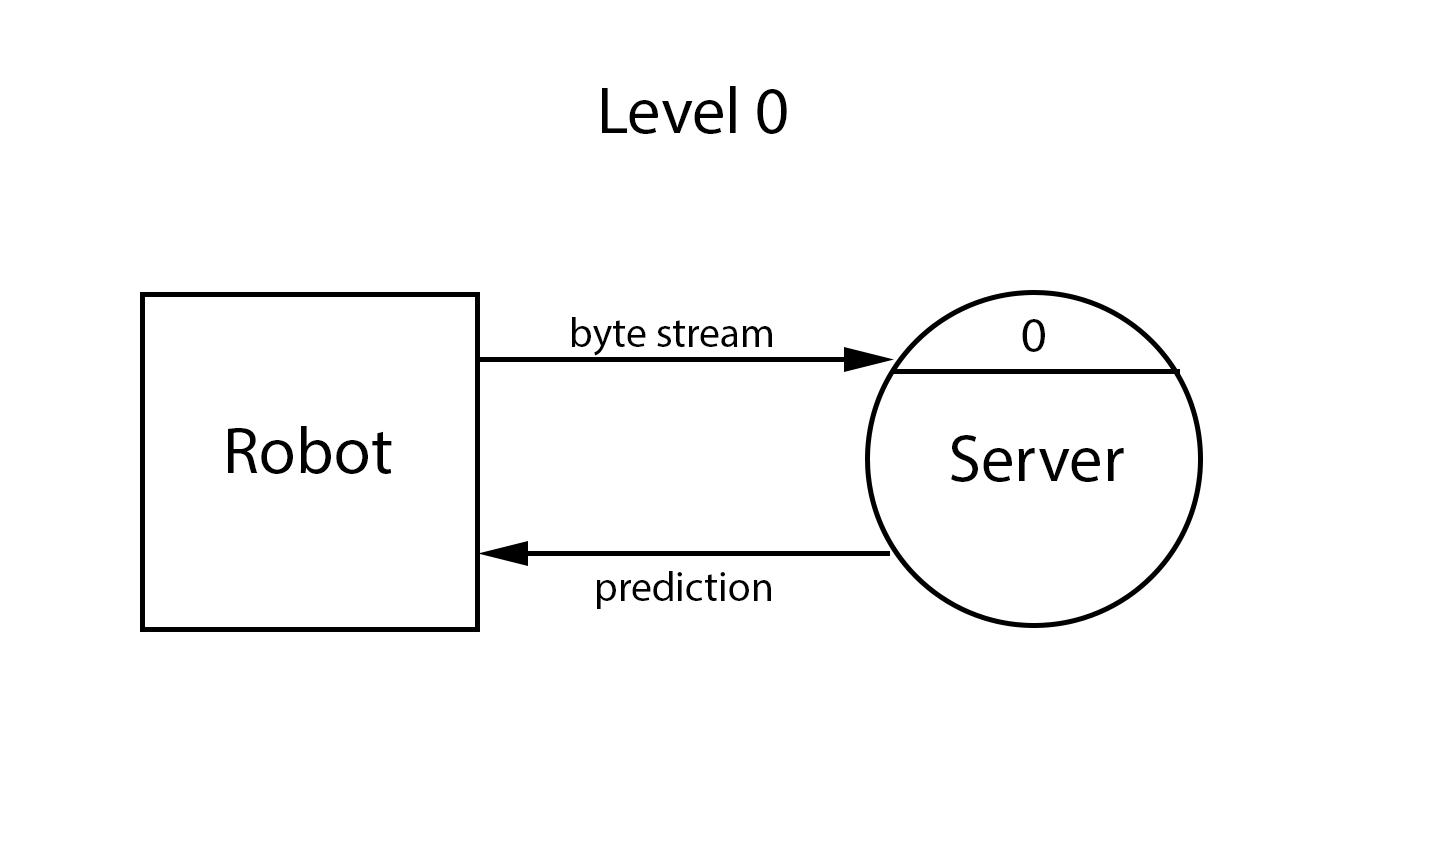
\includegraphics[scale=1.2]{level_0_dia.jpg}}
\end{flushleft}
\subsection{Data Flow Diagram - Level 1}
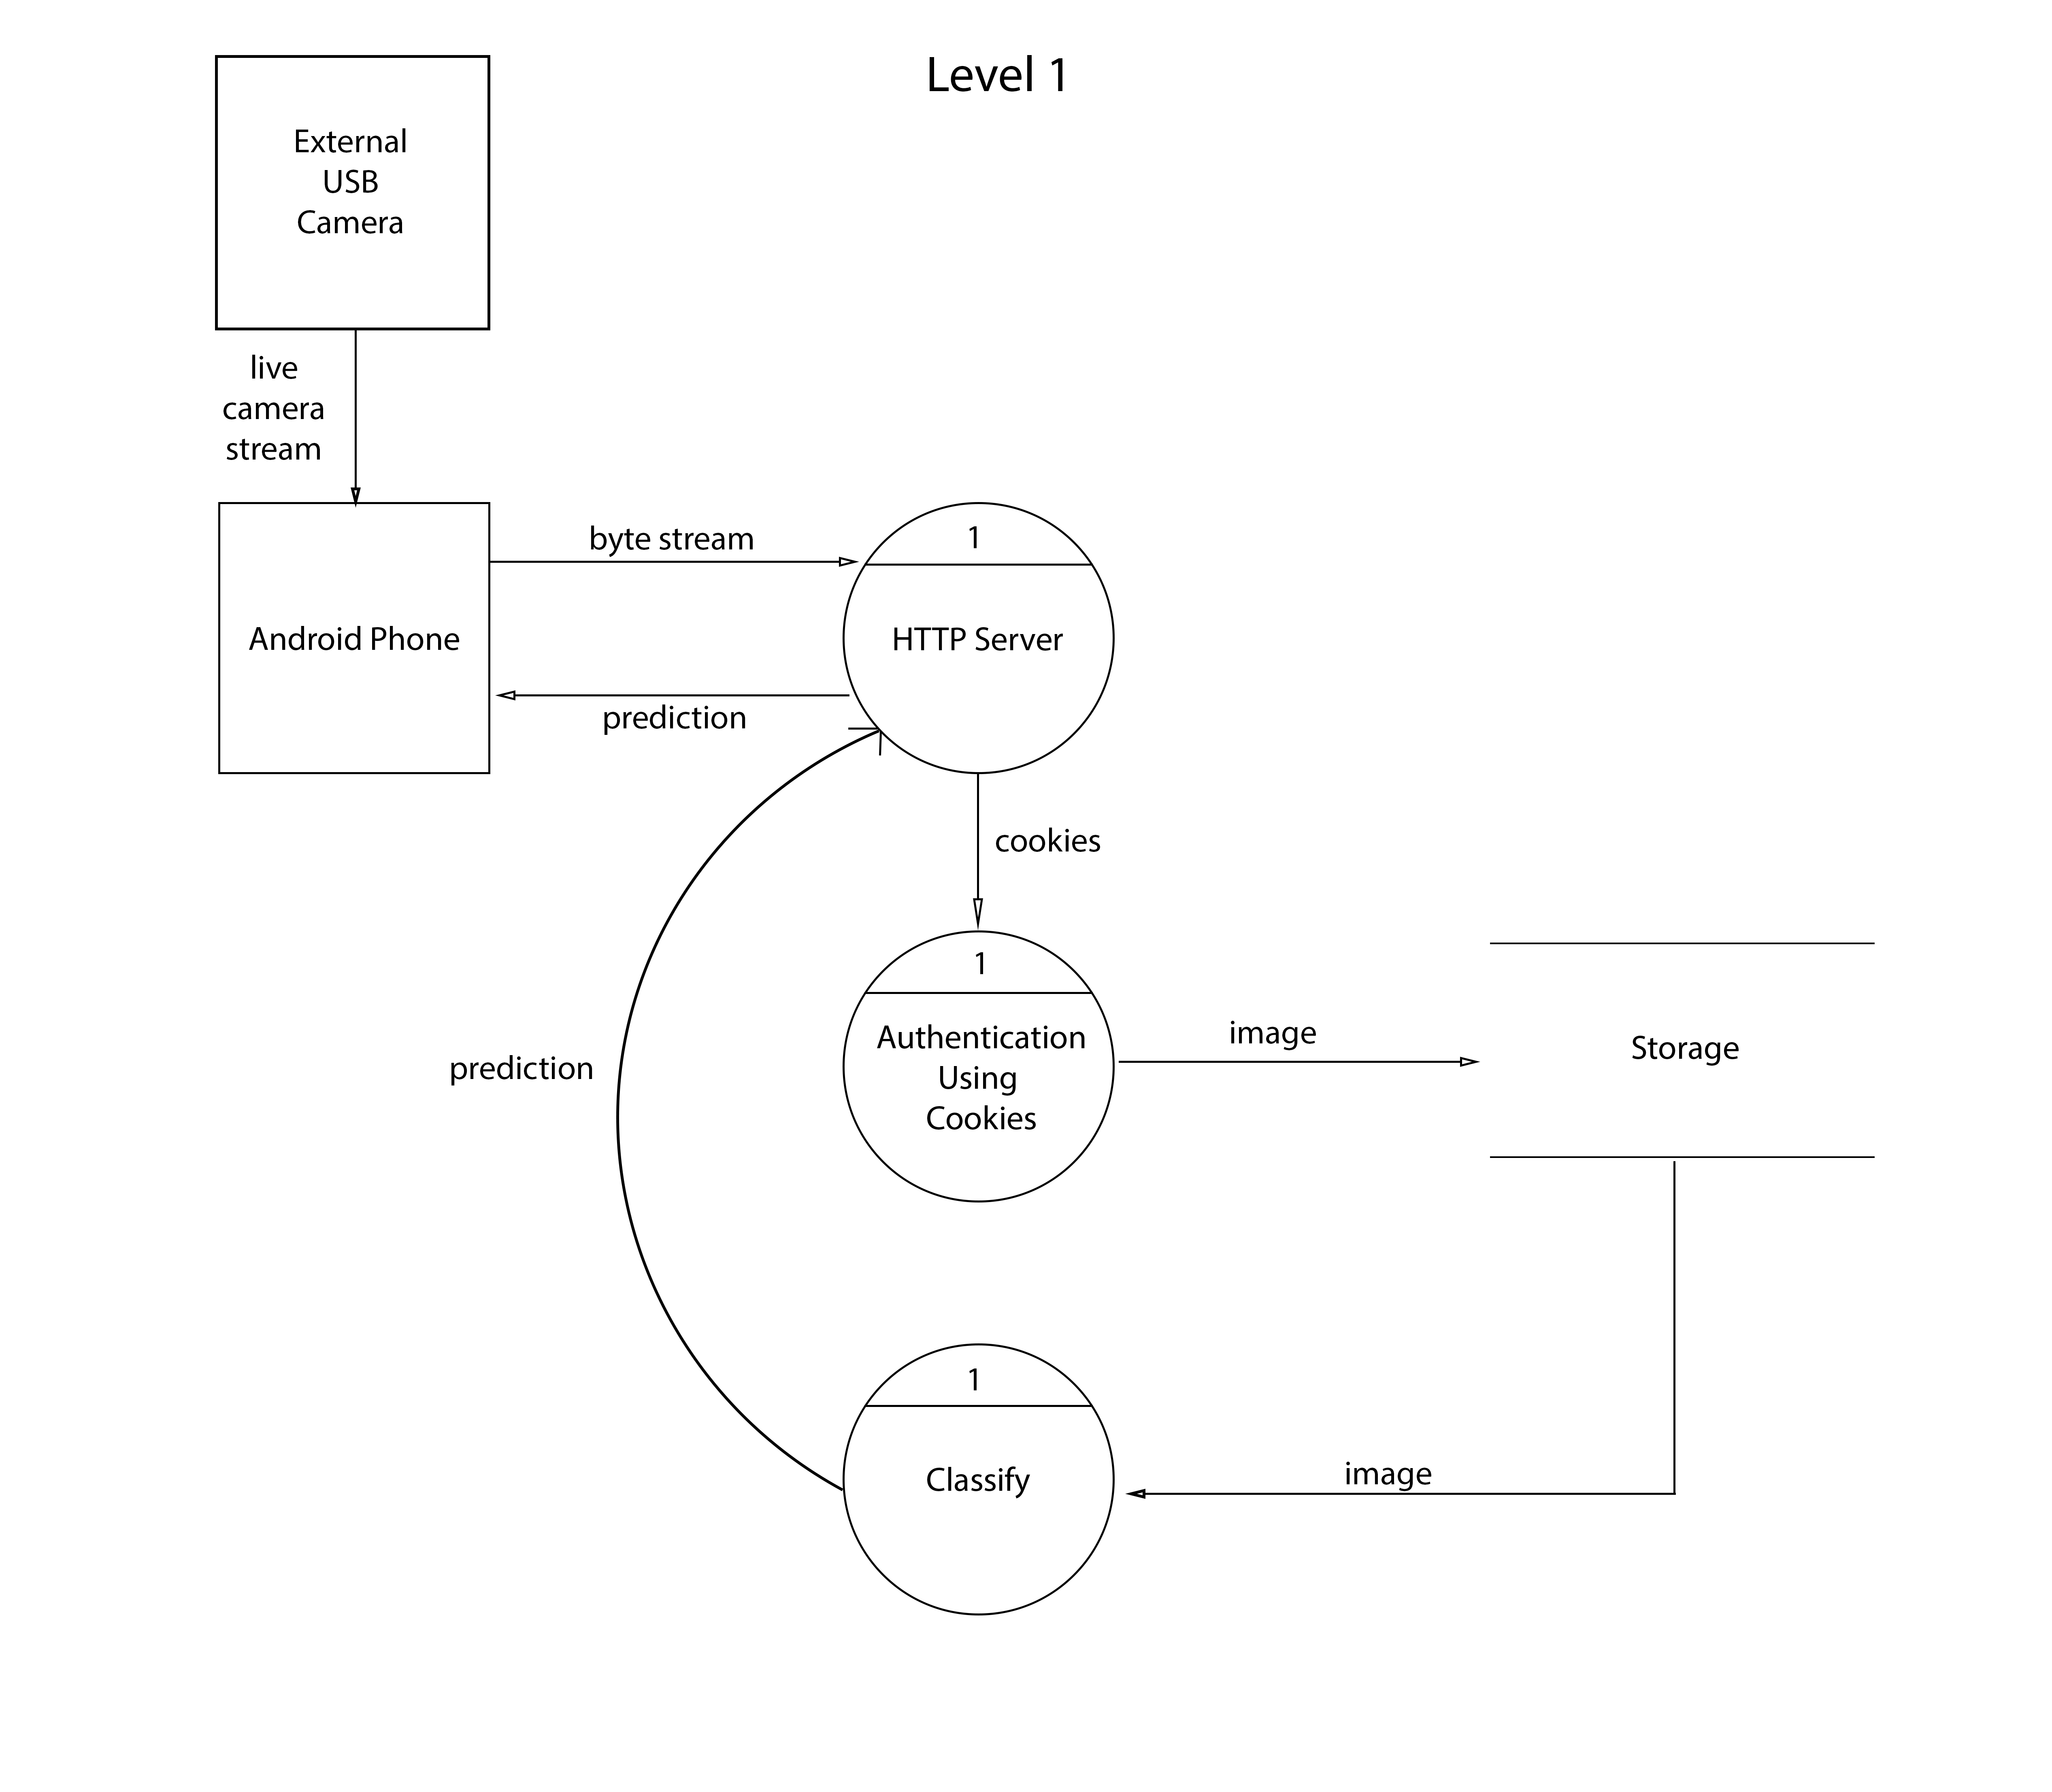
\includegraphics[scale=0.40]{level_1_dia.jpg}
\newpage
\subsection{3D-Designed Model}
\begin{figure}[H]
\centerline{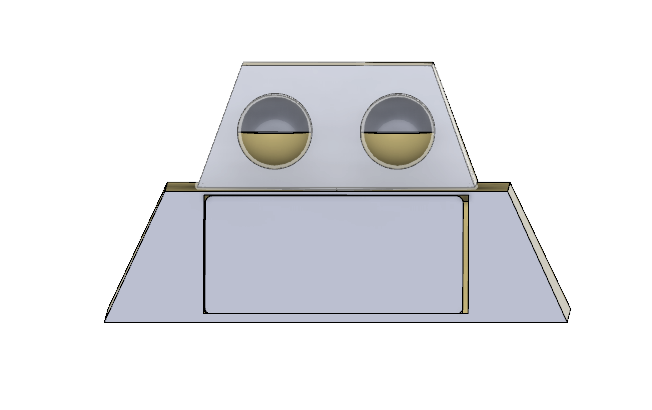
\includegraphics[scale=0.70]{sad.PNG}}
\caption{Front view of the robot}
\end{figure}
\begin{figure}[H]
\centerline{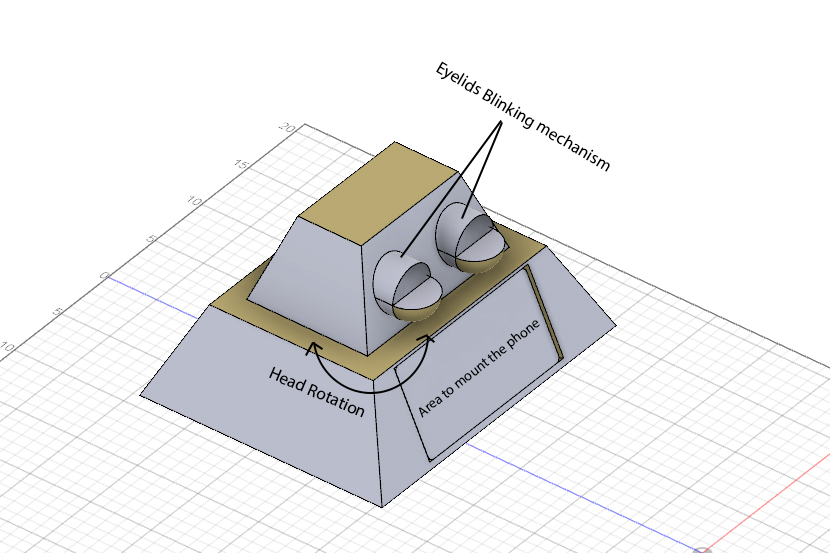
\includegraphics[scale=0.70]{side_label.jpg}}
\caption{Movements of the robot}
\end{figure}
\newpage
\section{Support Vector Machine(SVM)}
In machine learning, support vector machines\cite{l} (SVMs, also support vector networks) are supervised learning models with associated learning algorithms that analyze data used for classification and regression analysis. Given a set of training examples, each marked as belonging to one or the other of two categories, an SVM training algorithm builds a model that assigns new examples to one category or the other, making it a non-probabilistic binary linear classifier (although methods such as Platt scaling exist to use SVM in a probabilistic classification setting). An SVM model is a representation of the examples as points in space, mapped so that the examples of the separate categories are divided by a clear gap that is as wide as possible. New examples are then mapped into that same space and predicted to belong to a category based on which side of the gap they fall.\newline\newline
In addition to performing linear classification, SVMs can efficiently perform a non-linear classification using what is called the kernel trick, implicitly mapping their inputs into high-dimensional feature spaces.\newline
\begin{flushleft}
The main reasons why we used SVM over other popular image classification techniques is because:
\end{flushleft}
\begin{itemize}
	\item Training a model using SVM doesn't require that much computational power compared to deep learning and ANN models.
	\item HOG + SVM combination provides the best possible accuracy and performance among the supervised learning techniques.
	\item SVMs deliver a unique solution, since the optimality problem is convex. This is an advantage compared
to Neural Networks, which have multiple solutions associated with local minima and for this reason may
not be robust over different samples. 
\end{itemize}

\section{System Requirements}
\subsection{Hardware Requirements}
   \begin{enumerate}
       \item Arduino
       \item Mega servo motor
       \item Mini servo motor
       \item USB Camera
       \item Smart Phone
   \end{enumerate}
\subsection{Software Requirements}
   \begin{enumerate}
       \item Image Classification Modules
       \begin{enumerate}
            \item opencv
            \item sklearn
            \item numpy
            \item scipy
            \item scikit-learn
            \item h5py
        \end{enumerate}
       
       \item Server Modules
       \begin{enumerate}
           \item python-tornado
       \end{enumerate}
       
       \item Dataset Collection Modules
       \begin{enumerate}
           \item scrapy
       \end{enumerate}
       
       \item Android Modules
       \begin{enumerate}
            \item Retrofit 2
            \item UVC Camera
            \item GOTEV(speech)
       \end{enumerate}
       
       \item Arduino Control Modules
       \begin{enumerate}
            \item PyFirmata
            \item Firmata Protocol code for APL
       \end{enumerate}
    \end{enumerate}

\section{Implementation}
A simple flow of control can be described as follows:\newline\newline
The usb camera provides vision of the robot and this data is fetched by the android phone which then sends the data stream to the server, where classification takes place and the prediction is send back to the android app itself, and then the prediction is spoken out.\newline\newline
On a deeper level the implementation part can be divided into several stages.
\begin{itemize}
    \item Dataset Collection
    \item Android App Development
    \item Server Creation
    \item Creation Of Image Classification Model
    \item Hardware Side Modelling and Creation
    \item Hardware Control
\end{itemize}
\subsection{Dataset Collection}
The datasets were collected by creating a web crawler, that crawled sites like amazon, flipkart and other sites which had stock photos in large numbers. The crawler was created using the Scrapy library. The datasets were organized automatically into their respective directories(where directory name was the class label) using a python script. In total each of the class labels consisted of nearly 3500 images.
\subsection{Android App Development}
The android phone acts as a middle-ware between the robot and the server. The UVCCamera library was used to retrieve the live stream from the usb camera. Retrofit, a type safe REST Client library, was used in communicating with the server and most importantly for sending and receiving data from the server. The usb camera stream was converted to byte stream and it was sent to the server along with a unique id, which can act as the cookie, to the http server. The server sends back the predictions based on the data and it's received in the android app itself. This prediction is then spoken out using the Speech library.
\subsection{Server Creation}
An http server was created using the python-tornado library. The server can handle multiple users at a time. Most importantly, the server makes use of the image classification model to predict on the received data and send back the prediction to the client(which is the android app). The trained image classification model stored in the server will detect objects within a few milli seconds.
\subsection{Image Classification}
The Support Vector Machine(SVM) algorithm was used to train a image classification model. This classification technique was applied in training by making use of the inbuilt functions from the Sklearn library in python. Feature extraction using the concept of Histogram of Oriented Gradients(HOG) was implemented using opencv library. The pre-processing of the data(that is scaling and normalizing) was done using sklearn itself. For choosing the best hyper-parameters, GridSearch Tuning was also implemented. The encoded labels and all were stored in h5py files, which acted as containers, datasets and groups and allowed for easier debugging as well classification. Finally the trained image classification model is stored to the file system for later usage.
\subsection{Hardware Implementation}
The body of the social robot was made using Multi-Wood, which is a white sheet made up of 'U' Pvc polyester resin, as it's more easily moldable and handy. A usb camera was mount inside the head of the robot, and it acted as the eyes of the robot. The external eye and eyelids were 3D-printed for precision. Rotation of head and eyelids were done using servo motors. A total of 3 servo motors, 1 for rotating the head and 2 for blinking of eyelids were used.
\subsection{Hardware Control}
Arduino Uno was made to control the overall movement of the servo motors. The control signals for arduino were sent from python, by making use of the pyserial and pyfirmata libraries. The rotation of head, and closing of eyes were synchronized using python itself. The important part, which was making the robot face towards a "person/human" in its vision, was also done by synchronizing the movements based on the predictions made.
\newpage
\subsection{Libraries}
OpenCV : OpenCV has more than 2500 optimized algorithms, which includes a comprehensive set of both classic and state-of-the-art computer vision and machine learning algorithms. These algorithms can be used to detect and recognize faces, identify objects, classify human actions in videos, track camera movements, track moving objects, extract 3D models of objects, produce 3D point clouds from stereo cameras, stitch images together to produce a high resolution image of an entire scene, find similar images from an image database, remove red eyes from images taken using flash, follow eye movements, recognize scenery and establish markers to overlay it with augmented reality, etc.\cite{g}\newline\newline
Numpy : Numpy is a library for the Python programming language, adding support for large, multi-dimensional arrays and matrices, along with a large collection of high-level mathematical functions to operate on these arrays.\cite{g}\newline\newline
Sklearn and Scikit-learn : Scikit-learn (formerly scikits.learn) is a free software machine learning library for the Python programming language. It features various classification, regression and clustering algorithms including support vector machines, random forests, gradient boosting, k-means and DBSCAN, and is designed to inter-operate with the Python numerical and scientific libraries NumPy and SciPy.\cite{j}\newline\newline
Retrofit : Retrofit is a REST Client for Java and Android. It makes it relatively easy to retrieve and upload JSON (or other structured data) via a REST based webservice. In Retrofit we can configure which converter is used for the data serialization. Typically for JSON you use GSon, but we can add custom converters to process XML or other protocols. Retrofit uses the OkHttp library for HTTP requests.\cite{k}\newline\newline
UVCCamera : It's a native script to get access to UVC web camera on non-rooted Android devices and do further processing with the data stream.\cite{k}
\newline\newline


\chapter{TESTING}
Testing was done at several stages of the project. It was mainly used in choosing the best feature extraction method, in choosing a language for controlling arduino and for a server that can handle multiple users at a time.
\section{Feature Extraction Methods}
\begin{longtable}{ | p{5cm} | p{5cm} | p{5cm} |}
      \hline
      \textbf{Test Method} & \textbf{Expected Outcome} & \textbf{Outcome}\\
      \hline
      HOG & Counts occurrences of gradient orientation in localized portions of an image & Accurate feature descriptors were obtained\\
      \hline
      SURF and SIFT & Keypoint detection and description & Key points were detected, but the algorithms were not used since they are not free to use(patended)\\
      \hline
      HU-MOMENTS & Outline or “silhouette” of an object in an image & The feature descriptor was not enough for an accurate prediction\\
      \hline
\caption{Testing of Feature Extraction Methods}
\label{table:1}
\end{longtable}

\section{Arduino Controlling Methods}
\begin{longtable}{ | p{5cm} | p{5cm} | p{5cm} |}
      \hline
      \textbf{Test Method} & \textbf{Expected Outcome} & \textbf{Outcome}\\
      \hline
      Arduino Programming Language(APL) & Control each and every movement of the servo motors and overall synchronization & Not as expected. Dynamic control of the servos is not possible\\
      \hline
      Python(Standalone) & Dynamic Control and ease of use & Was more dynamic, but since the servos are controlled through a serial port, sending multiple control signals simultaneously proved erroneous\\
      \hline
      Python + APL & Accurate synchronization and control of servos & The firmata protocol allowed parallel executions and use of external libraries from python, combined with a start-up code from APL\\
      \hline
\caption{Testing of Arduino Controlling Methods}
\label{table:2}
\end{longtable}

\section{Asynchronous Networking}
\begin{longtable}{ | p{5cm} | p{5cm} | p{5cm} |}
      \hline
      \textbf{Test Method} & \textbf{Expected Outcome} & \textbf{Outcome}\\
      \hline
      Python-Flask & Ease of use & Limited in handling multiple requests at a time\\
      \hline
      Python-Tornado & Asynchronous Networking and speed & Was able to handle upto 10 users at a time simultaneously, without compromise in speed.\\
      \hline
\caption{Testing of Asynchronous Networking Methods}
\label{table:3}
\end{longtable}

\chapter{RESULTS}
The output of the project is a social robot which can identify the objects seen in its vision. The robot, in its physical structure, has a 180 degree view made possible by its head movements.\newline\newline
The robot performs a specific function of object classification. The live feed it retrieves from the usb camera attached to its eyes are fed to an android application on the phone. The app send the images to the server where it undergoes a number of processes as specified in the explanation of the project. Once the image classification is done, the result is displayed on the phone screen.\newline\newline
\begin{center}
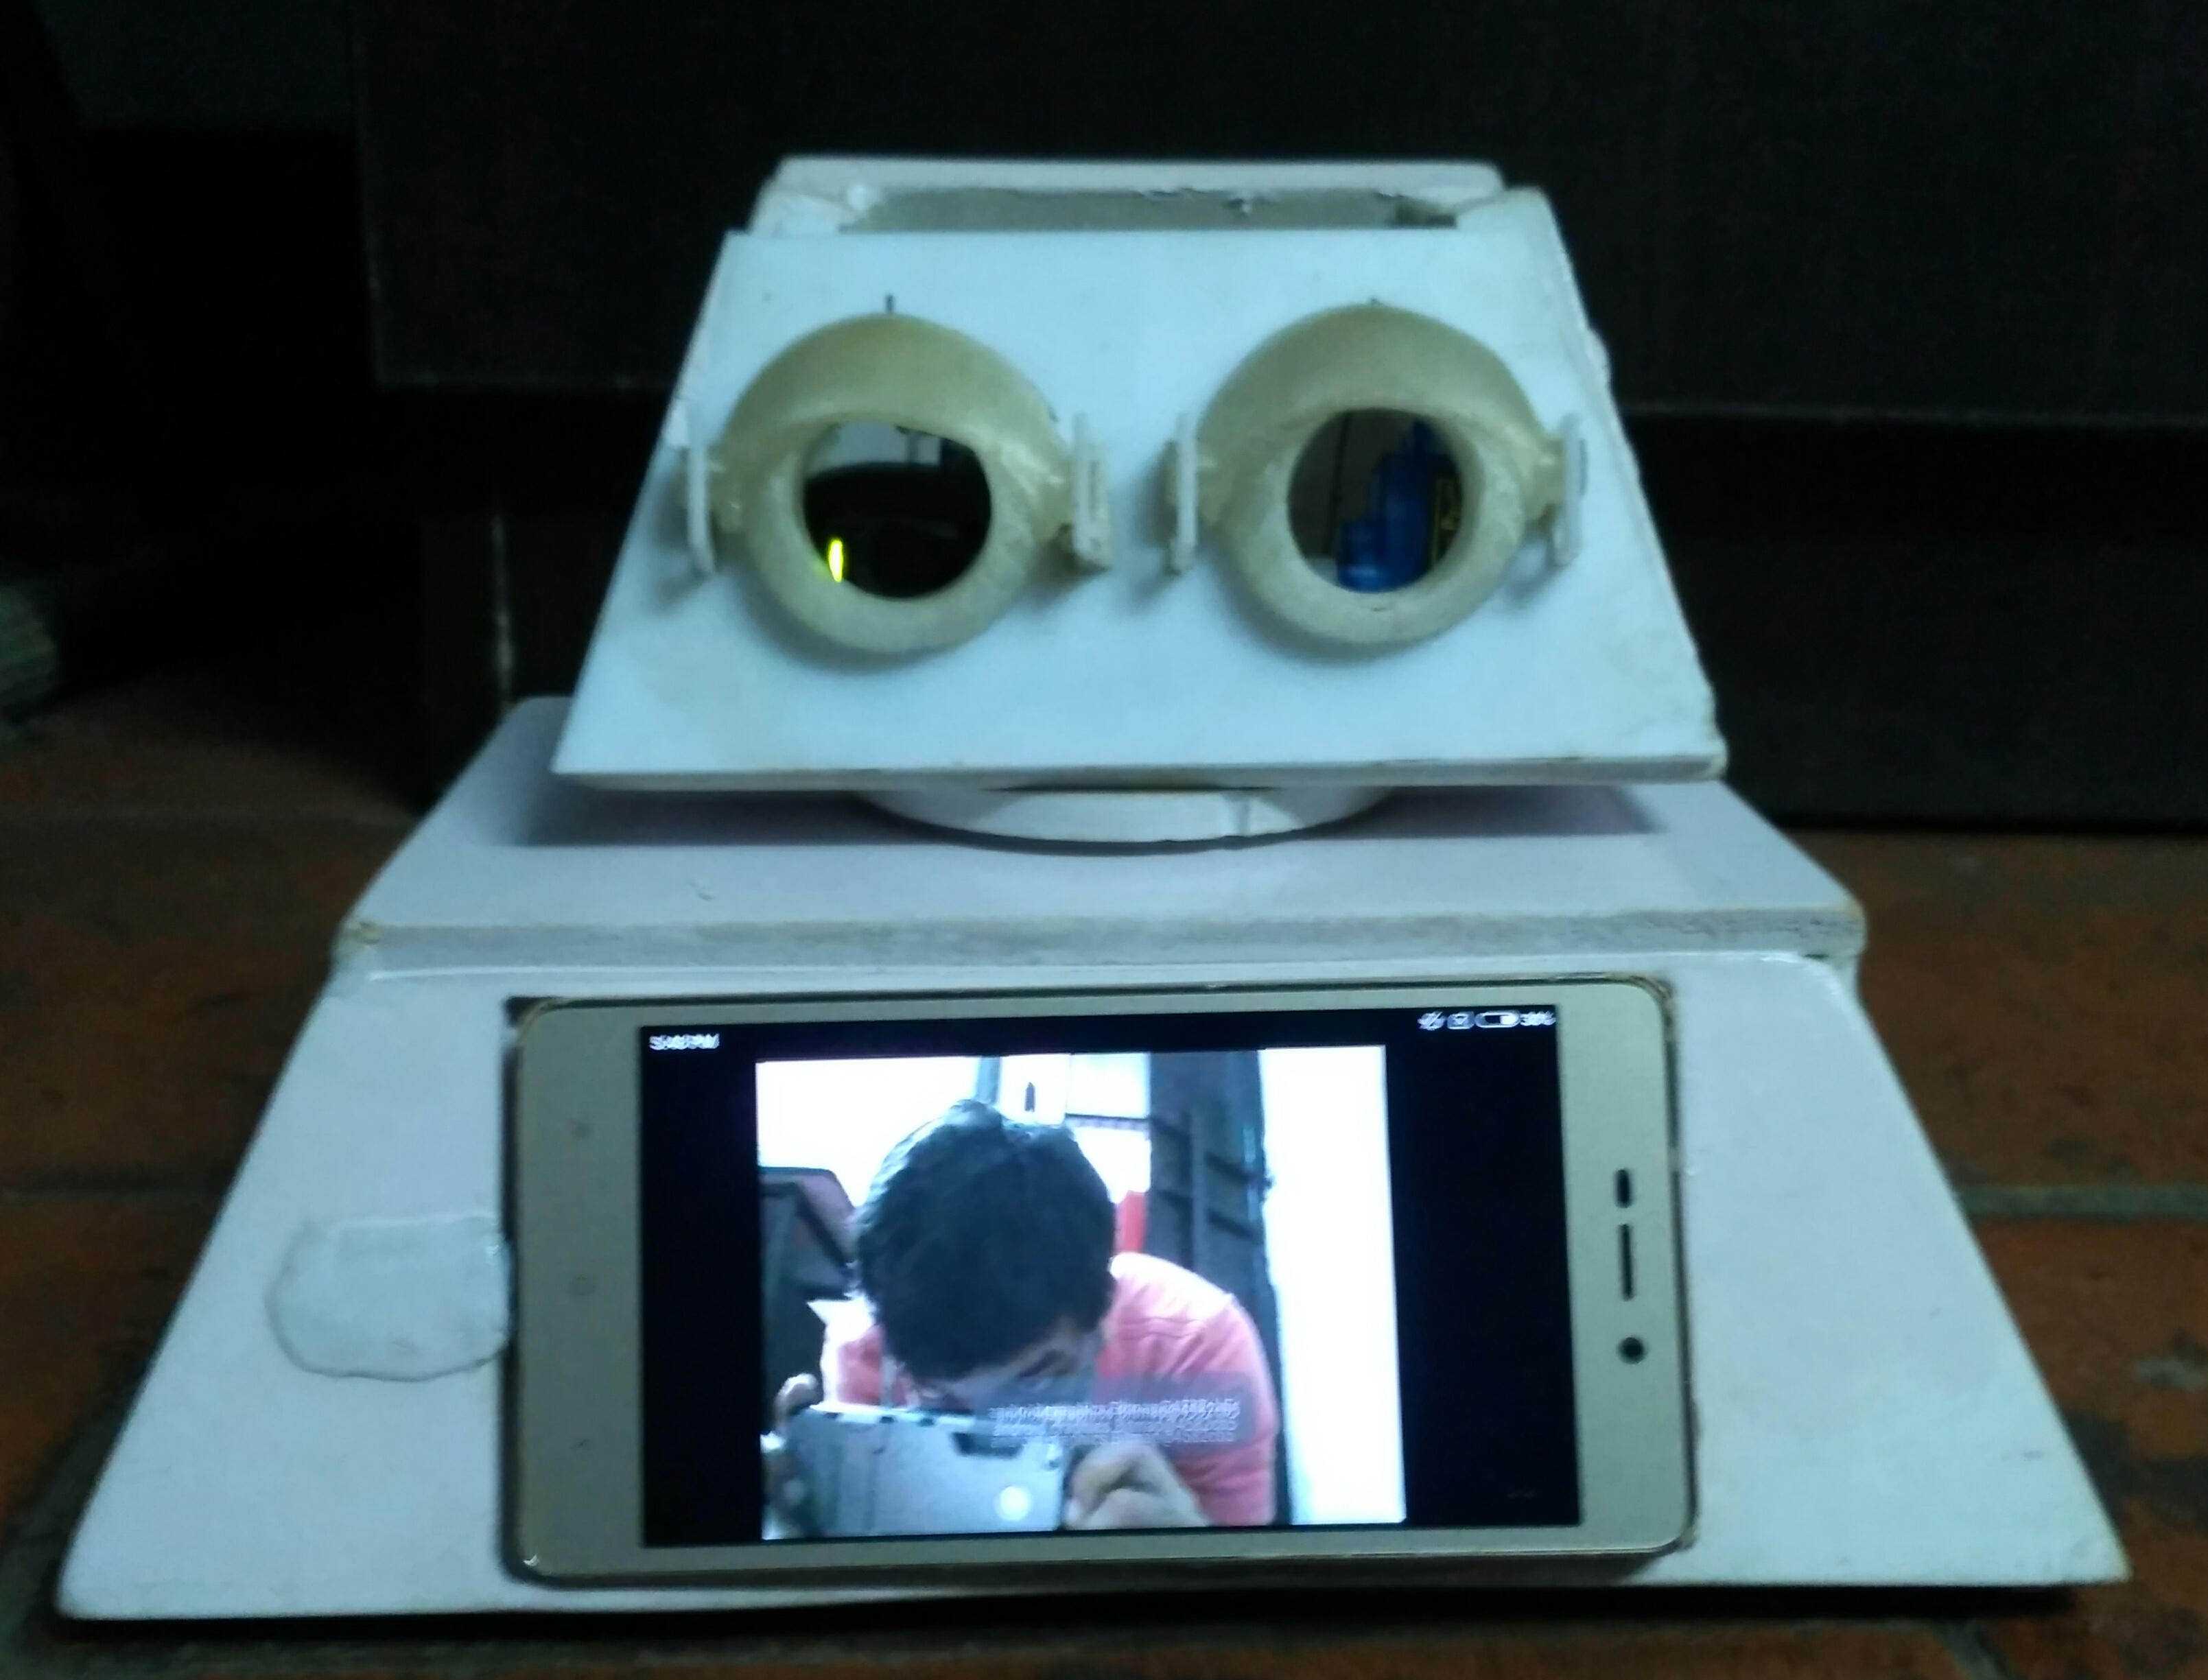
\includegraphics[scale=0.1]{real_front.jpg}
\captionof{figure}{Our Social Robot}
\end{center}   
\begin{center}
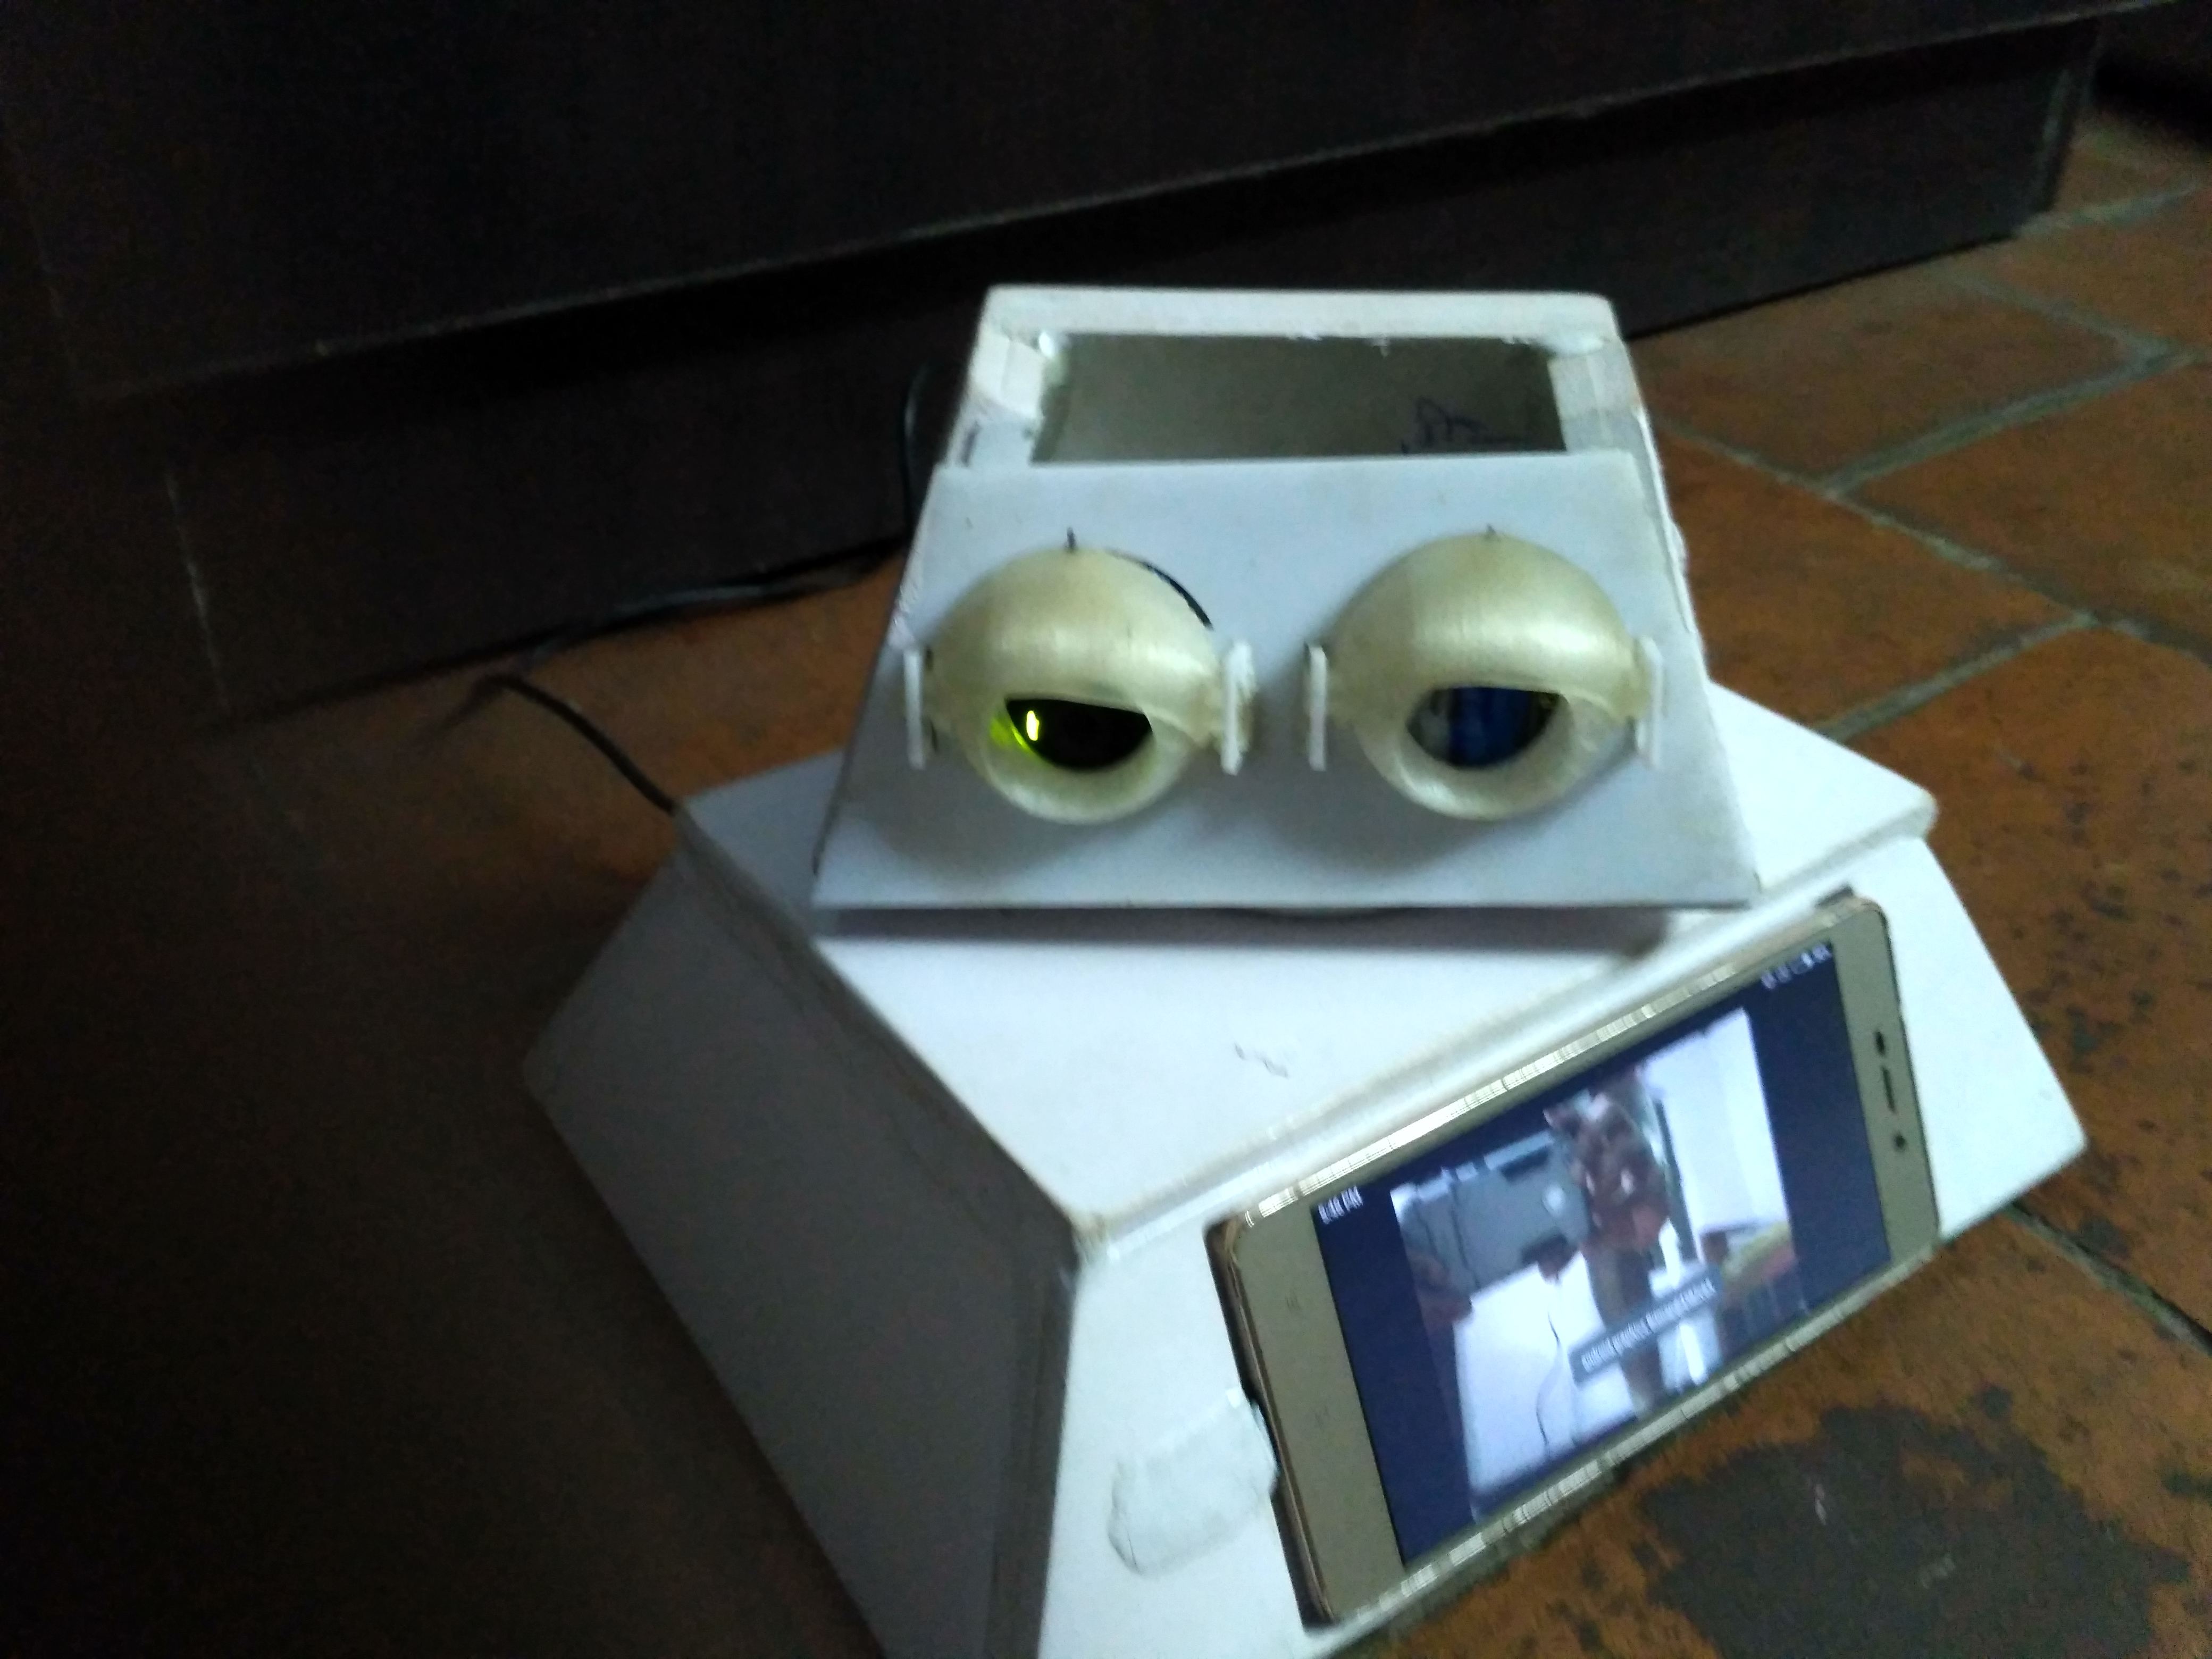
\includegraphics[scale=0.1]{real_side.jpg}
\captionof{figure}{Rotation of head}
\end{center}   
It has numerous civilian and military applications. But, on a undergrad level, what we aim to achieve is to bring high level of accuracy on live classification of objects and to incorporate with a physical model like a robot. What we can do with that, is according to its applications.

\chapter{CONTRIBUTIONS}
As I was the team leader, I had a definitive role to play in the overall completion of the project. I undertook many important responsibilities like getting the tasks done on time by using all of the available resources and co-ordinating with my teammates, for dividing and assigning tasks to teammates, for acting as the conduit between the college management, the teaching staff and my team, and most importantly played the role of a core developer in all stages and domains of the project.\newline\newline
The contributions made by each of the teammates were very much valuable to the completion of the project. Key contributions and roles made by each of the teammates is as follows :\newline
\begin{itemize}
	\item Ranjith R.K : Designed the 3D model, collected and organized the dataset, processed images and extracted features from it.
	\item Leo Varghese : Core developer in Android section of the project, implemented the ability to speak for the robot, sets up the vision of the robot, helped in crafting the hardware.
	\item Sandeep Ramesh : Implemented an image classification model using SVM and also helped in the hardware side.
\end{itemize}

\chapter{CONCLUSION}
A social robot is an autonomous robot that interacts and communicates with
humans or other autonomous physical agents by following social behaviors and
rules attached to its role.
This project successfully created a social robot, incorporated with human features such as, movement of head, closing of eyelids and speaking, and can identify and speak out about the objects seen through its vision, by making use of useful and popular computing techniques such as Android, Machine learning, Image processing and Servers.

\begin{thebibliography}{1}
\vspace{1cm}
\bibitem{a} 
Blackford, R. 2012. Robots and reality: A reply to Robert Sparrow. Ethics and Information Technology 14(1): 41–51.
\bibitem{b} 
Campa, Riccardo. 2015. Humans and automata. A social study of robotics. Frankfurt am Main: Peter Lang.
\bibitem{c}
Daerden, F., and D. Lefeber. 2000. Pneumatic artificial muscles: Actuators for robotics and automation. Vrije Universiteit Brussel.
\bibitem{d} 
Darling, Kate. 2012. Extending legal rights to social robots. Paper presented at We Robot Conference. University of Miami, April 23.
\bibitem{e}
Desai, J.P., G. Dudek, O. Khatib, and V. Kumar, eds. 2013. Experimental robotics. Heidelberg: Springer.
\bibitem{f} 
Flandorfer, Priska. 2012. Population ageing and socially assistive robots for elderly persons: The importance of sociodemographic factors for user acceptance. International Journal of Population Research Article ID 829835.
\bibitem{g} 
Floreano, D., and C. Mattiussi. 2008. Bio-inspired artificial intelligence: Theories, methods, and technologies. Cambridge, MA: MIT Press.
\bibitem{h}
Ge Shuzhi, S., H. Li, J.-J. Cabibihan, Y.K. Tan, eds. 2010. Social robotics. Second international conference. Proceedings. Heidelberg: Springer.
\bibitem{i}
Application of social robot:http://www.robotiksistem.com/robotics-applications.html
\bibitem{j}
Free software machine learning library for the Python programming language:https://scikit-learn.org/
\bibitem{k}
Android SDK tools and API documentation:https://developer.android.com/studio/
\bibitem{l}
Cortes, Corinna; Vapnik, Vladimir N. (1995). "Support-vector networks". Machine Learning. 20 (3): 273–297. doi:10.1007/BF00994018.
\end{thebibliography}

\begin{appendices}
\chapter{Feature Extraction Using HOG}
\begin{lstlisting}[language=python]
import cv2
import imutils
import storage as st
from trained_models import model

def histogram_of_oriented_gradients(image):
    winSize = (100, 100)
    blockSize = (10, 10)
    blockStride = (5, 5)
    cellSize = (10, 10)
    nbins = 9
    derivAperture = 1
    winSigma = -1.
    histogramNormType = 0
    L2HysThreshold = 0.2
    gammaCorrection = 1
    nlevels = 64
    signedGradients = True
    hog = cv2.HOGDescriptor(winSize, blockSize,
                            blockStride, cellSize,
                            nbins, derivAperture,
                            winSigma, histogramNormType,
                            L2HysThreshold, gammaCorrection,
                            nlevels, signedGradients)
    return hog.compute(image)

image = cv2.imread(st.__UPLOADS__+fname)
image = imutils.rotate_bound(image, 90)
#resize the image
image = cv2.resize(image, (100,100))
# convert to grayscale
image = cv2.cvtColor(image, cv2.COLOR_BGR2GRAY)
# extract features
gf = histogram_of_oriented_gradients(image)
# make prediction
prediction = model.predict(gf.reshape(1, -1))[0]
print(prediction)
\end{lstlisting}


\chapter{Support Vector Machines(SVM)}
\begin{lstlisting}[language=python]
from sklearn import svm
# we have, X (predictor) and Y (target) for training data set
# and x_test(predictor) of test_dataset
# Create SVM classification object 
model = svm.svc(kernel='linear', c=1, gamma=1) 
# there is various option associated with it, like changing kernel,
# gamma and C value.
# Train the model using the training sets and check score
model.fit(X, y)
model.score(X, y)
#Predict Output
predicted= model.predict(x_test)
\end{lstlisting}


\chapter{Retrofit POST Request API}
\begin{lstlisting}[language=java]
package com.ikigai.android.imageupload.apis;

import okhttp3.MultipartBody;
import okhttp3.RequestBody;
import okhttp3.ResponseBody;
import retrofit2.Call;
import retrofit2.http.Multipart;
import retrofit2.http.POST;
import retrofit2.http.Part;

public interface RetrofitInterface {
	@Multipart
	@POST("/upload")
	Call<ResponseBody> uploadImage(@Part MultipartBody.Part image);
}
\end{lstlisting}
\end{appendices}


\end{document}
